%!TEX program = xelatex
\documentclass[10pt]{beamer}

\usetheme[progressbar=frametitle]{metropolis}
\usepackage{appendixnumberbeamer}

\usepackage{booktabs}
\usepackage[scale=2]{ccicons}

\usepackage{bm}
\usepackage{amsmath,amsfonts}
\newcommand{\Tr}{\operatorname{Tr}}

\usepackage{subcaption}
\usepackage{natbib}

\usepackage{pgfplots}
\usepgfplotslibrary{dateplot}

\usepackage{xspace}
\newcommand{\themename}{\textbf{\textsc{metropolis}}\xspace}

\usepackage{graphicx}
\graphicspath{{../../../Figures/presentation_19_05/}{../../Figures/Report_19_09/}{../../Images/Report_19_09/}{"/Users/acfrery/Documents/Alunos/Danilo Fernandes/Figures/Report_19_09/Histograms/"}{"/Users/acfrery/Documents/Alunos/Danilo Fernandes/Figures/Report_19_09/"}{"/Users/acfrery/Documents/Alunos/Danilo Fernandes/Figures/Report_19_09/Parameters/"}{"/Users/acfrery/Documents/Alunos/Danilo Fernandes/Figures/Report_19_02_27/"}{"/Users/acfrery/Documents/Alunos/Danilo Fernandes/Images/Report_19_09/"}}

\title{Statistical Properties of Geodesic Distances between Samples and Elementary Scatterers in PolSAR Imagery}
% \date{\today}
\date{}
\author{Danilo Fernandes, Alejandro C. Frery}
\institute{Laboratório de Computação Científica e Análise Numérica\\ Universidade Federal de Alagoas}
% \titlegraphic{\hfill\includegraphics[height=1.5cm]{logo.pdf}}

\begin{document}

\maketitle

\begin{frame}{Table of contents}
  \setbeamertemplate{section in toc}[sections numbered]
  \tableofcontents%[hideallsubsections]
\end{frame}

\section[Intro]{Introduction}

\begin{frame}[fragile]{Introduction}

    In Polarimetric SAR, a radar target is characterized by a scattering matrix $\bm S$ that describes the dependence of its scattering properties on the polarization. 
    It is defined as
    \[\mathbf{S} = 
    \begin{bmatrix}
    S_{\text{HH}} & S_{\text{HV}}\\
    S_{\text{VH}} & S_{\text{VV}}\\
    \end{bmatrix}
    ,\]
    
    where $\text{H}$ and $\text{V}$ denote, respectively, horizontal and vertical polarization.
  
\end{frame}

\begin{frame}[fragile]{Introduction}

    Another important matrix in PolSAR theory is the coherency $\bm{T}$ obtained by:
    $$
    \mathbf{T} = \frac{1}{L}\sum_{i=1}^{L}k_{p_i}k_{p_i}^{T*},
    $$
    where $k_p = 2^{-1/2} 
    \begin{bmatrix}
    S_{\text{HH}} + S_{\text{VV}} &S_{\text{HH}} - S_{\text{VV}} &2S_{\text{HV}}
    \end{bmatrix}^T
    $, $T$ denotes transposition,  $*$ denotes the complex conjugate, and $L$ is the number of looks.

\end{frame}

\begin{frame}[fragile]{Introduction}
  An approach to representing the PolSAR information in a real matrix is by the Kennaugh matrix. A Kennaugh matrix $\mathbf{K}$ can be obtained from the coherency matrix $\mathbf{T}$ in the following manner:
\[\mathbf{K} = 
\begin{bmatrix}
\frac{ T_{11} + T_{22} + T_{33} }{2} & \Re(T_{12}) & \Re(T_{13}) & \Im(T_{23})\\
\Re(T_{12}) & \frac{T_{11} + T_{22} - T_{33}}{2} & \Re(T_{23}) & \Im(T_{13})\\
\Re(T_{13}) & \Re(T_{23}) & \frac{ T_{11} - T_{22} + T_{33} }{2} & -\Im(T_{12})\\
\Im(T_{23}) & \Im(T_{13}) & -\Im(T_{12}) & \frac{ -T_{11} + T_{22} + T_{33} }{2}\\
\end{bmatrix}
.\]
\end{frame}

\begin{frame}[fragile]{Introduction}
    One way to measure the distance between two Kennaugh matrices $\bm K_1$ and $\bm K_2$ is through the Geodesic Distance, which is given by~\cite{ClassificationPolSARGeodesic}: 
    \begin{displaymath}
    \text{GD}(\mathbf{K_1}, \mathbf{K_2}) = \frac{2}{\pi} \cos^{-1} \left(\frac{\Tr(\mathbf{K_1}^T \mathbf{K_2})}{\sqrt{\Tr(\mathbf{K_1}^T \mathbf{K_1})} \sqrt{\Tr(\mathbf{K_2}^T \mathbf{K_2}})} \right),
    \end{displaymath}
    where $\Tr$ denotes the trace. It ranges between $[0,1]$. 
    Consequently, a similarity can be defined as 
    $$
    f(K_1, K_2) = 1 - GD(K_1, K_2).$$
    
    The audience has already seen \alert{deterministic} results, properties, and applications of this approach.
\end{frame}

\begin{frame}{Next question}

\begin{alertblock}{What do we see in practice?}
In practice, we should always expect some degree of variation/deviation from the ideal/noiseless situation.

With this in mind,
\begin{itemize}
	\item Which are the statistical properties of the similarity of actual targets to ideal Kennaugh matrices?
	\item Can we use such properties to convert data into knowledge?
\end{itemize}
\end{alertblock}
\end{frame}

\begin{frame}{First attempt}
Initially, we took samples in a merely visual manner.

Although careful, this na\"ive approach did not produce good insights.

This kind of statistical analysis requires carefully collected and validated samples.
\end{frame}

\begin{frame}{The data}
	\begin{figure}[hbt]
		\centering
		\subcaptionbox{16 May 2016\label{fig:r1}}{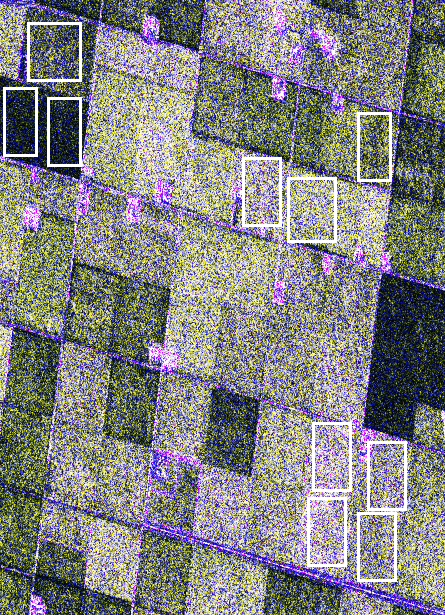
\includegraphics[width = .19\linewidth]{/Regions/regions_1}}
		\subcaptionbox{09 June 2016\label{fig:r2}}{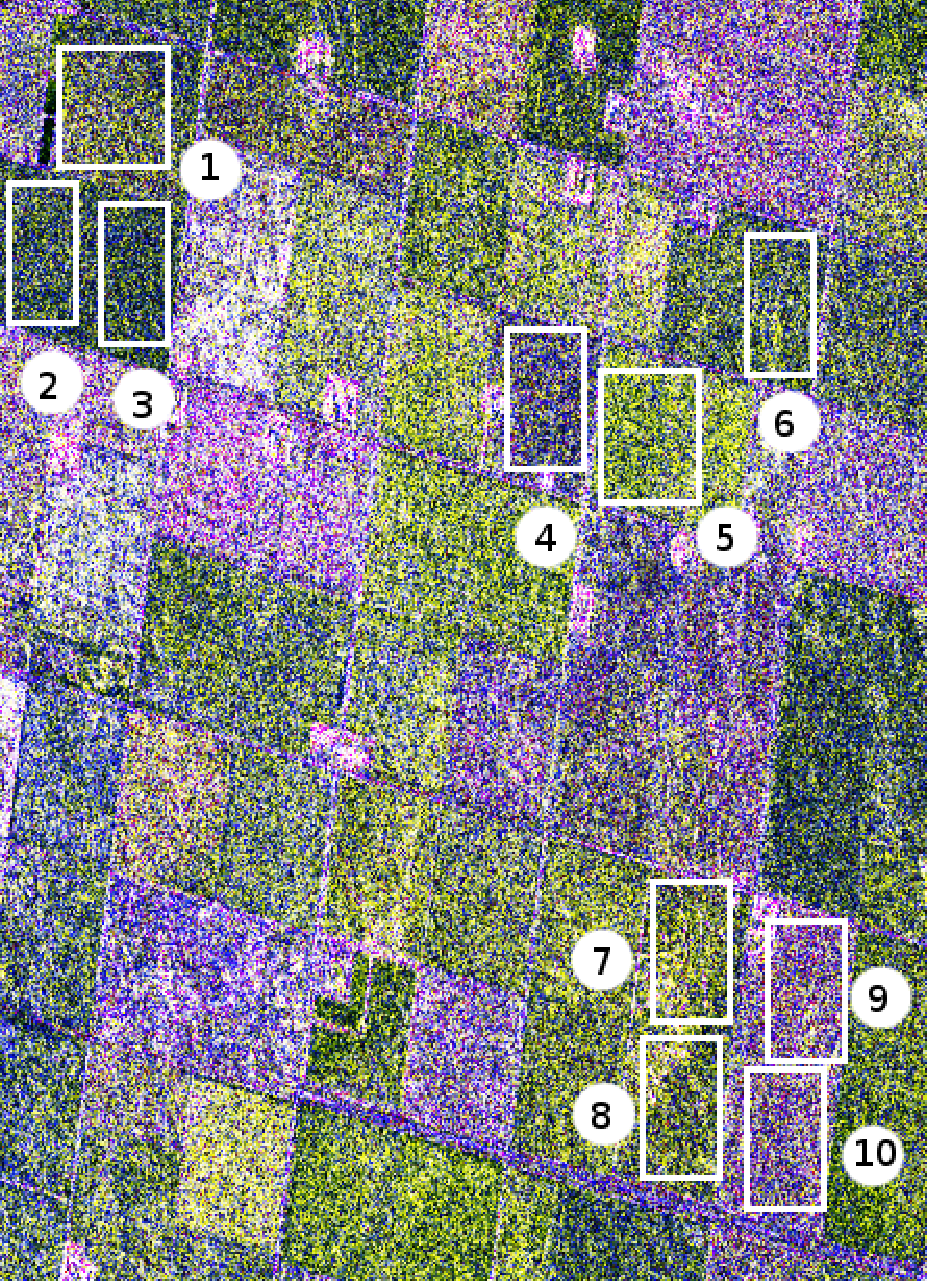
\includegraphics[width = .19\linewidth]{/Regions/regions_2}}
		\subcaptionbox{03 July 2016\label{fig:r3}}{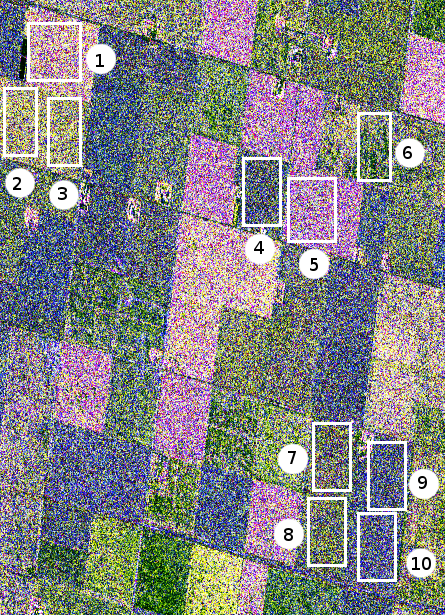
\includegraphics[width = .19\linewidth]{/Regions/regions_3}}
		\subcaptionbox{27 July 2016\label{fig:r4}}{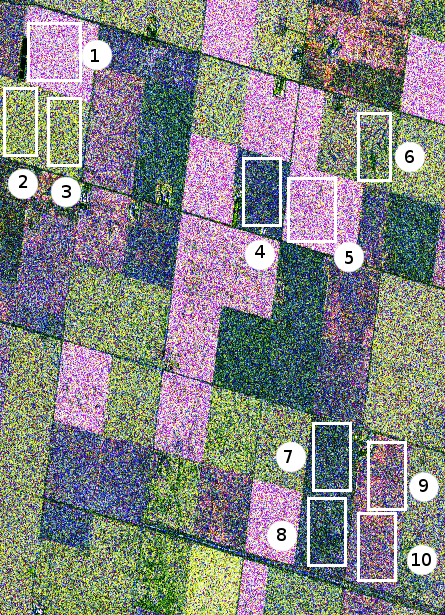
\includegraphics[width = .19\linewidth]{/Regions/regions_4}}
		\subcaptionbox{20 Aug. 2016\label{fig:r5}}{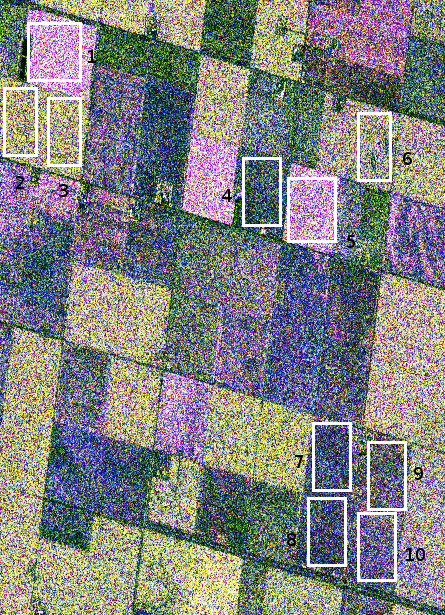
\includegraphics[width = .19\linewidth]{/Regions/regions_5}}
		\caption{Samples analyzed over time: 1 to 10 corresponding, respectively, to Canola 43, Soybeans 231, Soybeans 232, Wheat 225, Canola 224, Soybeans 101, Oats 102, Oats 103, Wheat 105 and Wheat 104}
	\end{figure}
\end{frame}

\begin{frame}{The model}
We employed the Beta model, and estimated the parameters by maximum likelhood.

\begin{table}[hbt]
	\centering
	\caption{$p$-values of the Kolmogorov-Smirnov goodness-of-fit test of the distances to trihedral an random volume}\label{tab:pvalues_table}
{\tiny 	\begin{tabular}{lrrrrrrrrrr}
		\toprule
		& \multicolumn{2}{c}{16 May 2016} & \multicolumn{2}{c}{09 June 2016} & \multicolumn{2}{c}{03 July 2016} & \multicolumn{2}{c}{27 July 2016} & \multicolumn{2}{c}{20 Aug. 2016}\\
		& TR & RV & TR & RV & TR & RV & TR & RV& TR & RV\\
		\cmidrule(lr){2-11}
		\textbf{SB 101} & 0.065 & 0.517 & 0.947 & 0.758 & \textbf{0.059} & 0.195 & 0.452 & 0.109 & 0.401 & 0.144\\
		\textbf{SB 231} & 0.775 & 0.242 & 0.573 & 0.166 & 0.314 & 0.275 & 0.239 & 0.114 & 0.416 & 0.070\\
		\textbf{SB 232} & 0.244 & 0.340 & 0.968 & 0.328 & 0.713 & 0.070 & 0.422 & 0.357 & 0.163 & 0.630\\
		\textbf{WT 104} & 0.178 & 0.715 & 0.421 & 0.094 & 0.514 & 0.779 & 0.062 & 0.369 & 0.602 & 0.919\\
		\textbf{WT 105} & 0.231 & 0.090 & 0.069 & 0.139 & 0.557 & 0.613 & 0.108 & 0.195 & 0.192 & 0.252\\
		\textbf{WT 255} & 0.235 & 0.513 & 0.270 & 0.375 & 0.628 & 0.279 & 0.653 & 0.069 & 0.437 & \textbf{0.993}\\
		\textbf{CN 43}  & 0.238 & 0.406 & 0.217 & 0.202 & 0.930 & 0.318 & 0.623 & 0.732 & 0.262 & 0.747\\
		\textbf{CN 224} & 0.184 & 0.116 & 0.128 & 0.333 & 0.298 & 0.714 & 0.813 & 0.409 & 0.305 & 0.391\\
		\textbf{OT 102} & 0.289 & 0.191 & 0.243 & 0.532 & 0.384 & 0.212 & 0.710 & 0.370 & 0.928 & 0.396\\
		\textbf{OT 103} & 0.096 & 0.139 & 0.139 & 0.186 & 0.265 & 0.079 & 0.936 & 0.079 & 0.989 & 0.489\\
		\bottomrule
	\end{tabular}}
\end{table}
\end{frame}


\section[Histograms]{Histograms of similarities in relation to elementary targets}

\subsection{Soybeans}

\begin{frame}{Soybeans versus trihedral and random volume}
\begin{figure}[hbt]
	\centering
	\subcaptionbox{16 May 2016}{\includegraphics[width = .19\linewidth]{/Histograms/1th_observation/Soybeans_101/histogram_trihedral_1}}
	\subcaptionbox{09 June 2016}{\includegraphics[width = .19\linewidth]{/Histograms/2th_observation/Soybeans_101/histogram_trihedral_2}}
	\subcaptionbox{03 July 2016}{\includegraphics[width = .19\linewidth]{/Histograms/3th_observation/Soybeans_101/histogram_trihedral_3}}
	\subcaptionbox{27 July 2016}{\includegraphics[width = .19\linewidth]{/Histograms/4th_observation/Soybeans_101/histogram_trihedral_4}}
	\subcaptionbox{20 Aug. 2016}{\includegraphics[width = .19\linewidth]{/Histograms/5th_observation/Soybeans_101/histogram_trihedral_5}}
	\caption{Histograms of the Geodesic Distances between trihedral and the pixels of the sample extracted from Soybeans 101 most similar to trihedral}
	\label{fig:sb101_hist_tri}
\end{figure}

\begin{figure}[hbt]
	\centering
	\subcaptionbox{16 May 2016}{\includegraphics[width = .19\linewidth]{/Histograms/1th_observation/Soybeans_101/histogram_random_volume_1}}
	\subcaptionbox{09 June 2016}{\includegraphics[width = .19\linewidth]{/Histograms/2th_observation/Soybeans_101/histogram_random_volume_2}}
	\subcaptionbox{03 July 2016}{\includegraphics[width = .19\linewidth]{/Histograms/3th_observation/Soybeans_101/histogram_random_volume_3}}
	\subcaptionbox{27 July 2016}{\includegraphics[width = .19\linewidth]{/Histograms/4th_observation/Soybeans_101/histogram_random_volume_4}}
	\subcaptionbox{20 Aug. 2016}{\includegraphics[width = .19\linewidth]{/Histograms/5th_observation/Soybeans_101/histogram_random_volume_5}}
	\caption{Histograms of the Geodesic Distances between random volume and the pixels of the sample extracted from Soybeans 101 most similar to random volume}
	\label{fig:sb101_hist_rv}
\end{figure}
\end{frame}

\subsection{Wheat}

\begin{frame}{Wheat 104 versus trihedral and random volume}
\begin{figure}[hbt]
	\centering
	\subcaptionbox{16 May 2016}{\includegraphics[width = .19\linewidth]{/Histograms/1th_observation/Wheat_104/histogram_trihedral_1}}
	\subcaptionbox{09 June 2016}{\includegraphics[width = .19\linewidth]{/Histograms/2th_observation/Wheat_104/histogram_trihedral_2}}
	\subcaptionbox{03 July 2016}{\includegraphics[width = .19\linewidth]{/Histograms/3th_observation/Wheat_104/histogram_trihedral_3}}
	\subcaptionbox{27 July 2016}{\includegraphics[width = .19\linewidth]{/Histograms/4th_observation/Wheat_104/histogram_trihedral_4}}
	\subcaptionbox{20 Aug. 2016}{\includegraphics[width = .19\linewidth]{/Histograms/5th_observation/Wheat_104/histogram_trihedral_5}}
	\caption{Histograms of the Geodesic Distances between trihedral and the pixels of the sample extracted from Wheat 104 most similar to trihedral}
	\label{fig:wt104_hist_tri}
\end{figure}

\begin{figure}[hbt]
	\centering
	\subcaptionbox{16 May 2016}{\includegraphics[width = .19\linewidth]{/Histograms/1th_observation/Wheat_104/histogram_random_volume_1}}
	\subcaptionbox{09 June 2016}{\includegraphics[width = .19\linewidth]{/Histograms/2th_observation/Wheat_104/histogram_random_volume_2}}
	\subcaptionbox{03 July 2016}{\includegraphics[width = .19\linewidth]{/Histograms/3th_observation/Wheat_104/histogram_random_volume_3}}
	\subcaptionbox{27 July 2016}{\includegraphics[width = .19\linewidth]{/Histograms/4th_observation/Wheat_104/histogram_random_volume_4}}
	\subcaptionbox{20 Aug. 2016}{\includegraphics[width = .19\linewidth]{/Histograms/5th_observation/Wheat_104/histogram_random_volume_5}}
	\caption{Histograms of the Geodesic Distances between random volume and the pixels of the sample extracted from Wheat 104 most similar to random volume}
	\label{fig:wt104_hist_rv}
\end{figure}
\end{frame}

\subsection{Canola}

\begin{frame}{Canola 43 versus trihedral and random volume}
	\begin{figure}[hbt]
		\centering
		\subcaptionbox{16 May 2016}{\includegraphics[width = .19\linewidth]{/Histograms/1th_observation/Canola_43/histogram_trihedral_1}}
		\subcaptionbox{09 June 2016}{\includegraphics[width = .19\linewidth]{/Histograms/2th_observation/Canola_43/histogram_trihedral_2}}
		\subcaptionbox{03 July 2016}{\includegraphics[width = .19\linewidth]{/Histograms/3th_observation/Canola_43/histogram_trihedral_3}}
		\subcaptionbox{27 July 2016}{\includegraphics[width = .19\linewidth]{/Histograms/4th_observation/Canola_43/histogram_trihedral_4}}
		\subcaptionbox{20 Aug. 2016}{\includegraphics[width = .19\linewidth]{/Histograms/5th_observation/Canola_43/histogram_trihedral_5}}
		\caption{Histograms of the Geodesic Distances between trihedral and the pixels of the sample extracted from Canola 43 most similar to trihedral}
		\label{fig:cn43_hist_tri}
	\end{figure}

\begin{figure}[hbt]
	\centering
	\subcaptionbox{16 May 2016}{\includegraphics[width = .19\linewidth]{/Histograms/1th_observation/Canola_43/histogram_random_volume_1}}
	\subcaptionbox{09 June 2016}{\includegraphics[width = .19\linewidth]{/Histograms/2th_observation/Canola_43/histogram_random_volume_2}}
	\subcaptionbox{03 July 2016}{\includegraphics[width = .19\linewidth]{/Histograms/3th_observation/Canola_43/histogram_random_volume_3}}
	\subcaptionbox{27 July 2016}{\includegraphics[width = .19\linewidth]{/Histograms/4th_observation/Canola_43/histogram_random_volume_4}}
	\subcaptionbox{20 Aug. 2016}{\includegraphics[width = .19\linewidth]{/Histograms/5th_observation/Canola_43/histogram_random_volume_5}}
	\caption{Histograms of the Geodesic Distances between random volume and the pixels of the sample extracted from Canola 43 most similar to random volume}
	\label{fig:cn43_hist_rv}
\end{figure}
\end{frame}

\subsection{Oats}

\begin{frame}{Oats versus trihedral and random volume}
\begin{figure}[hbt]
	\centering
	\subcaptionbox{16 May 2016}{\includegraphics[width = .19\linewidth]{/Histograms/1th_observation/Oats_102/histogram_trihedral_1}}
	\subcaptionbox{09 June 2016}{\includegraphics[width = .19\linewidth]{/Histograms/2th_observation/Oats_102/histogram_trihedral_2}}
	\subcaptionbox{03 July 2016}{\includegraphics[width = .19\linewidth]{/Histograms/3th_observation/Oats_102/histogram_trihedral_3}}
	\subcaptionbox{27 July 2016}{\includegraphics[width = .19\linewidth]{/Histograms/4th_observation/Oats_102/histogram_trihedral_4}}
	\subcaptionbox{20 Aug. 2016}{\includegraphics[width = .19\linewidth]{/Histograms/5th_observation/Oats_102/histogram_trihedral_5}}
	\caption{Histograms of the Geodesic Distances between trihedral and the pixels of the sample extracted from Oats 102 most similar to trihedral}
	\label{fig:ot102_hist_tri}
\end{figure}

\begin{figure}[hbt]
	\centering
	\subcaptionbox{16 May 2016}{\includegraphics[width = .19\linewidth]{/Histograms/1th_observation/Oats_102/histogram_random_volume_1}}
	\subcaptionbox{09 June 2016}{\includegraphics[width = .19\linewidth]{/Histograms/2th_observation/Oats_102/histogram_random_volume_2}}
	\subcaptionbox{03 July 2016}{\includegraphics[width = .19\linewidth]{/Histograms/3th_observation/Oats_102/histogram_random_volume_3}}
	\subcaptionbox{27 July 2016}{\includegraphics[width = .19\linewidth]{/Histograms/4th_observation/Oats_102/histogram_random_volume_4}}
	\subcaptionbox{20 Aug. 2016}{\includegraphics[width = .19\linewidth]{/Histograms/5th_observation/Oats_102/histogram_random_volume_5}}
	\caption{Histograms of the Geodesic Distances between random volume and the pixels of the sample extracted from Oats 102 most similar to random volume}
	\label{fig:ot102_hist_rv}
\end{figure}

\begin{figure}[hbt]
	\centering
	\subcaptionbox{16 May 2016}{\includegraphics[width = .19\linewidth]{/Histograms/1th_observation/Oats_102/histogram_trihedral_1}}
	\subcaptionbox{09 June 2016}{\includegraphics[width = .19\linewidth]{/Histograms/2th_observation/Oats_102/histogram_trihedral_2}}
	\subcaptionbox{03 July 2016}{\includegraphics[width = .19\linewidth]{/Histograms/3th_observation/Oats_102/histogram_trihedral_3}}
	\subcaptionbox{27 July 2016}{\includegraphics[width = .19\linewidth]{/Histograms/4th_observation/Oats_102/histogram_trihedral_4}}
	\subcaptionbox{20 Aug. 2016}{\includegraphics[width = .19\linewidth]{/Histograms/5th_observation/Oats_102/histogram_trihedral_5}}
	\caption{Histograms of the Geodesic Distances between trihedral and the pixels of the sample extracted from Oats 102 most similar to trihedral}
	\label{fig:ot102_hist_tri}
\end{figure}
\end{frame}

\begin{frame}{Histogramas das similaridades em relação aos retroespalhadores elementares}
	\begin{figure}
		\centering
		\includegraphics[width = .6\linewidth]{rv.pdf}
		\caption{Similaridade entre os dados PolSAR de regiões de vegetação e solo exposta em relação ao retroespalhador elementar \textit{random volume}}
		\label{fig:rv}
	\end{figure}
\end{frame}

\section{Temporal analysis}

\begin{frame}{Do we see any temporal change?}
\begin{figure}
  \subcaptionbox{Soybeans 231\label{subfig:tri_mean_sb231}}{\includegraphics[width = .45\linewidth]{/Parameters/mean_tri_over_time_sb231}}
\subcaptionbox{Soybeans 232\label{subfig:tri_mean_sb232}}{\includegraphics[width = .45\linewidth]{/Parameters/mean_tri_over_time_sb232}}
\caption{Mean of the distances between trihedral and samples extracted from Soybeans 231 and 232 over time}
%%% ACF Usar notch=TRUE, explicar e analisar: é um intervalo de confiança assintótico ao 95% da mediana
\label{fig:tri_mean_sb_231_232}
\end{figure}
\end{frame}

\section{Parameter Estimation}

\begin{frame}[fragile]{Estimation of the parameters of the Beta distribution and mean for the analysed similarities}
    \begin{table}[hbt]
    \centering
    %\caption{}\label{tab:estimated_params}     
    \begin{tabular}{lrrrrr}
    \toprule
    & $\min$ & $\max$ & $\widehat\alpha$ & $\widehat\beta$ & $\widehat\mu$\\ \midrule
    & \multicolumn{5}{c}{$-1/4$-wave}\\
    \cmidrule(lr){2-6}
    \textbf{Forest} & 0.000 & 1.000 & 7.830 & 22.758 & 0.255\\
    \textbf{Bare soil} & 0.055 & 0.400 & 1.127 & 4.872 & 0.119\\
    \midrule
    %
    & \multicolumn{5}{c}{$+1/4$-wave}\\
    \cmidrule(lr){2-6}
    \textbf{Forest} & 0.000 & 1.000 & 8.681 & 23.277 & 0.271\\
    \textbf{Bare soil} & 0.090 & 0.450 & 1.200 & 4.800 & 0.162\\
    \midrule
    %
    & \multicolumn{5}{c}{Cylinder}\\
    \cmidrule(lr){2-6}
    \textbf{Forest} & 0.000 & 1.000 & 7.500 & 12.165 & 0.381\\
    \textbf{Bare soil} & 0.140 & 0.600 & 1.243 & 4.756 & 0.235\\
    \bottomrule
    \end{tabular}
    \end{table}
\end{frame}

\begin{frame}[fragile]{Estimation of the parameters of the Beta distribution and mean for the analysed similarities}
    \begin{table}[hbt]
    \centering
    %\caption{}\label{tab:estimated_params}     
    \begin{tabular}{lrrrrr}
    \toprule
    & $\min$ & $\max$ & $\widehat\alpha$ & $\widehat\beta$ & $\widehat\mu$\\ \midrule
    & \multicolumn{5}{c}{Dihedral}\\
    \cmidrule(lr){2-6}
    \textbf{Forest} & 0.000 & 1.000 & 5.380 & 36.870 & 0.127\\
    \textbf{Bare soil} & 0.009 & 0.070 & 1.327 & 4.672 & 0.022\\
    \midrule
    %
    & \multicolumn{5}{c}{Dipole}\\
    \cmidrule(lr){2-6}
    \textbf{Forest} & 0.000 & 1.000 & 8.358 & 22.658 & 0.269\\
    \textbf{Bare soil} & 0.075 & 0.350 & 1.625 & 4.374 & 0.149\\
    \midrule
    %
    & \multicolumn{5}{c}{Narrow dihedral}\\
    \cmidrule(lr){2-6}
    \textbf{Forest} & 0.000 & 1.000 & 5.890 & 33.198 & 0.150\\
    \textbf{Bare soil} & 0.016 & 0.150 & 1.119 & 4.880 & 0.041\\
    \bottomrule
    \end{tabular}
    \end{table}
\end{frame}

\begin{frame}[fragile]{Estimation of the parameters of the Beta distribution and mean for the analysed similarities}
    \begin{table}[hbt]
    \centering
    %\caption{}\label{tab:estimated_params}     
    \begin{tabular}{lrrrrr}
    \toprule
    & $\min$ & $\max$ & $\widehat\alpha$ & $\widehat\beta$ & $\widehat\mu$\\ \midrule
    & \multicolumn{5}{c}{Left helix}\\
    \cmidrule(lr){2-6}
    \textbf{Forest} & 0.000 & 1.000 & 27.408 & 96.013 & 0.222\\
    \textbf{Bare soil} & 0.000 & 1.000 & 8.380 & 24.286 & 0.256\\
    \midrule
    & \multicolumn{5}{c}{Right helix}\\
    \cmidrule(lr){2-6}
    \textbf{Forest} & 0.000 & 1.000 & 28.522 & 71.238 & 0.285\\
    \textbf{Bare soil} & 0.000 & 1.000 & 8.316 & 20.574 & 0.287\\
    \midrule
    %
    & \multicolumn{5}{c}{Random volume}\\
    \cmidrule(lr){2-6}
    \textbf{Forest} & 0.000 & 1.000 & 20.074 & 11.910 & \textcolor{red}{0.627}\\
    \textbf{Bare soil} & 0.360 & 0.800 & 1.218 & 4.781 & \textcolor{red}{0.449}\\
    \bottomrule
    \end{tabular}
    \end{table}
\end{frame}

\begin{frame}[fragile]{Estimation of the parameters of the Beta distribution and mean for the analysed similarities}
    \begin{table}[hbt]
    \centering
    %\caption{}\label{tab:estimated_params}     
    \begin{tabular}{lrrrrr}
    \toprule
    & $\min$ & $\max$ & $\widehat\alpha$ & $\widehat\beta$ & $\widehat\mu$\\ \midrule
    & \multicolumn{5}{c}{Trihedral}\\
    \cmidrule(lr){2-6}
    \textbf{Forest} & 0.000 & 1.000 & 7.197 & 9.996 & 0.418\\
    \textbf{Bare soil} & 0.150 & 0.650 & 1.408 & 4.592 & 0.267\\
    \bottomrule
    \end{tabular}
    \end{table}
\end{frame}

\section[Goodness-of-fit test]{p-values obtained by Kolmogorov-Smirnov goodness-of-fit test}

\begin{frame}{p-values obtained by Kolmogorov-Smirnov goodness-of-fit test}
    \begin{table}[hbt]
    \centering
    %\caption{$p$-values of the Kolmogorov-Smirnov goodness-of-fit test of the similarity w.r.t. elementary backscatterers}\label{tab:pvalues_table}
    \begin{tabular}{lrrrrr}
    \toprule
    & $-1/4$- & $+1/4$- & Cylinder & Dihedral & Dipole\\
    & wave & wave & & &\\
    \cmidrule(lr){2-6}
    \textbf{Forest} & 0.979 & 0.808 & 0.763 & 0.733 & 0.975\\
    \textbf{Bare soil} & 0.361 & 0.893 & 0.264 & 0.443 & 0.475\\
    \midrule
    & Left & Narrow & Random & Right & Trihedral\\
    & helix & dihedral & volume & helix & \\
    \cmidrule(lr){2-6}
    \textbf{Forest} & 0.959 & 0.787 & 0.589 & 0.344 & 0.582\\
    \textbf{Bare soil} & 0.099 & 0.206 & 0.480 & 0.072 & 0.127\\
    \bottomrule
    \end{tabular} 
    \end{table}
\end{frame}

\subsection{Contato}
\begin{frame}
	\begin{alertblock}{Contact}
		Alejandro C.\ Frery\\
		\texttt{acfrery@laccan.ufal.br}\\
		\url{http://lattes.cnpq.br/2312365155234431}\\
		\url{http://www.researcherid.com/rid/A-8855-2008}\\
	\end{alertblock}
	\centering
	\includegraphics[width=5cm]{laccan.pdf}\\
\end{frame}	

\begin{frame}[allowframebreaks]{References}
\nocite{ANovelRadarVegetationIndexforCompactPolarimetricSARData2019,ClassificationPolSARGeodesic,AScatteringPowerFactorizationFrameworkUsingaGeodesicdistanceinRadarPolarimetry2018,AScatteringPowerFactorizationFrameworkUsingaGeodesicDistanceforMultilookedPolSARData2019,NovelTechniquesforBuiltupAreaExtractionfromPolarimetricSARImages2019,AGeneralizedVolumeScatteringModelBasedVegetationIndexfromPolarimetricSARData2019}
  \bibliographystyle{abbrv}
  \bibliography{rdt}

\end{frame}

\end{document}
